%\documentclass[pageno]{jpaper}
\documentclass[conference]{IEEEtran}

%\usepackage{natbib}
\usepackage[sort, numbers]{natbib}
\usepackage[normalem]{ulem}
%\usepackage{pseudocode}
\usepackage{algorithm}
%\usepackage{algorithmic}
\usepackage{verbatim}
\usepackage{epsfig}
\usepackage{graphicx}
\usepackage{amsmath}
\usepackage{comment}
\usepackage{multirow}
\usepackage{multicol}
\usepackage{textcomp}
\let\labelindent\relax
\usepackage{enumitem}
%\usepackage{authblk}
\begin{document}
%\setcitestyle{square}

%\newcommand\blfootnote[1]{%
%  \begingroup
%  \renewcommand\thefootnote{}\footnote{#1}%
%  \addtocounter{footnote}{-1}%
%  \endgroup
%}


%\title{Thermal-aware application mapping on a reconfigurable CMOS-TFET heterogeneous multicore}
\large
\title{Refresh Enabled Video Analytics (REVA): Implications on Power and Performance of DRAM Supported Embedded Visual Systems}
\normalsize

\author{ \IEEEauthorblockN{Siddharth Advani\IEEEauthorrefmark{1}, Nandhini Chandramoorthy\IEEEauthorrefmark{1}, Karthik Swaminathan\IEEEauthorrefmark{1}, \\ Kevin Irick\IEEEauthorrefmark{2}, Yeong Cheol Cho\IEEEauthorrefmark{3},  Jack Sampson\IEEEauthorrefmark{1} and Vijaykrishnan Narayanan\IEEEauthorrefmark{1}}
\IEEEauthorblockA{\IEEEauthorrefmark{1}Pennsylvania State University $\quad$ \IEEEauthorrefmark{2}Silicon Scapes LLC. $\quad$\IEEEauthorrefmark{3}ETRI, South Korea}}


\date{}
\maketitle

\thispagestyle{empty}

\begin{abstract}
\label{sec:abstract}	%0.25 col
Video applications are becoming ubiquitous in mobile and embedded systems. Wearable video systems such as Google glasses require capabilities for real-time video analytics and prolonged battery lifetimes for wide adoption. Further, the increasing resolution of image sensors in these mobile systems places an increasing demand on both the memory storage as well as the computational power. Consequently, there is growing interest in energy-efficient algorithms and hardware for video analytics. In this work, we present the \textbf{R}efresh \textbf{E}nabled \textbf{V}ideo \textbf{A}nalytics (REVA) system, an embedded architecture for multi-object scene understanding and tackle the unique opportunities provided by real-time embedded video analytics applications for reducing the DRAM memory refresh energy. We compare our design with the existing design space and show savings of 88.1\% in refresh power and 14.8\% in total power, as compared to a standard DRAM refresh scheme. Results indicate the benefits of utilizing "smart" energy-efficient memories in next-generation real-time visual systems. 

\end{abstract}

%\blfootnote {\textbf{978-3-9815370-2-4/DATE14/\textcopyright2014 EDAA}}
\section{Introduction}
%Introduction and motivation
\label{sec:introduction}			%1
Video applications are becoming ubiquitous in mobile and embedded systems. Wearable video systems such as Google glasses require capabilities for real-time video analytics and prolonged battery lifetimes for wide adoption.  Further, the increasing resolution of image sensors in these mobile systems places an increasing demand on both the memory storage as well as the computational power. Consequently, there is growing interest in energy-efficient algorithms and hardware for video analytics. 
Deriving inspiration from the energy-efficiency of the visual cortex, many brain-inspired algorithms and architectures have been proposed to support energy-efficient video analytics applications~\cite{Nere2011,Chen2014,Kestur2012,Maashri2012a,Farabet}. %[YiranChen UPitt, Qingriu Syracuse, NEC CNN]. 

In order to achieve fast and energy efficient implementations of these algorithms, it has been found general-purpose processors are inadequate, even with highly tuned software optimizations. Consequently, a host of application-specific accelerators are employed, allied with a general purpose core for other tasks such as synchronization and co-ordination between the individual specialized computation engines. 


Most works in this domain have focused mainly on enhancing the performance and energy efficiency of the computational fabrics and do not address the inefficiencies of the main memory system. The memory system contributes between 10-30\% of the overall power of embedded video systems and mobile phones~\cite{CarrollAaronHeiser2010}. 
%For instance, our system uses accelerators for realizing tasks such as object saliency, object recognition and action recognition in a fast and energy-efficient manner, with low area overhead. Ho
The increasing memory size in new generations of embedded systems and the use of stacked 3D architectures that increase on-chip temperatures have drawn increasing attention on reducing the memory refresh energy. Consequently, there have been sustained efforts to introduce new power-efficient techniques such as Low Power Auto Self Refresh, Temperature Controlled Refresh, Refresh Pausing, Fine Granularity Refresh and Data Bus Inversion in new memory standards such as DDR4~\cite{jedec-sdram-standards}.  However, software exploitation of these advanced hardware features has generally lagged~\ref{Mukundan2013,refresh-pausing-taco2014}. 
Tuning DRAM refresh based on the data characteristics has been proposed as early as 1998~\cite{islped98}. Recently, a software approach, termed as \emph{Flikker} was proposed that relies on the user to annotate critical and non-critical parts. This technique has been used to effectively exploit a modified version of the standard Partial Array Self Refresh (PASR) hardware mechanism~\cite{Liu2011}. It also allows refresh rates to be different for critical and non-critical sections of the memory and conserve the refresh energy. 
There have been several other works in the design of accelerator-based systems for vision analytics. For instance~\cite{Effex} proposes \emph{EFFEX}, a specialized heterogeneous multicore design for vision applications in the embedded domain. In this paper, the authors have proposed customizations to the memory hierarchy, such as hardware-software co-optimized patch memory architectures. However, the memory optimizations are mainly restricted to the software level and there remains substantial scope for optimizing the memory architecture itself, especially from the point of view of improving energy and bandwidth utilization.

In this work, we focus on the unique opportunities provided by real-time embedded video analytics applications for reducing the memory refresh energy. The analysis is based on an real-time image detection and recognition system that has been emulated on a FPGA based platform. This system detects objects of interest using an attention algorithm and then the object can be picked up from a subsequent frame where it is recognized to be of a particular class. The recognized object can be further passed to a next level for more detailed recognition. This system represents generic components in a wide variety of end applications in unmanned air-vehicles, security cameras, visual-aids for visually-impaired and automatic weapon systems. In this work, we make the following contributions with regard to reducing the memory refresh energy based of this video analytics application.

\begin{itemize}
\item First, we recognize that in streaming data, the lifetime of some parts of the data are significantly less than the refresh periods of a DRAM. Therefore, we completely disable refresh in these parts of the memory. This is an enhancement to current techniques that reduce refresh times instead of completely shutting off the refresh in non-critical portions of the data. We are also able to eliminate refresh for portions of the memory that are guaranteed to be accessed within a specific time period due to the application specific nature of the embedded video system.
\item Second, we are able to automatically recognize portions of an image as critical based on the saliency-recognition algorithms employed in brain-inspired vision algorithms and selectively refresh portions of data. This is contrast to prior efforts that have focused on manual annotations of critical and non-critical regions that limit such classification to be static. An example of such annotation in~\cite{Liu2011}, annotates the code and certain data structures such as pointers to list of frames as critical while consider the image data itself as non-critical. This approach limits the granularity of such annotations to a coarse-grain, especially when such criticality is data-driven. In contrast, our automated system can exploit both data dependent and task dependent information to identify salient regions within a single image frame. 
The human visual cortex filters a significant amount of the raw visual stimuli for further processing by using attention mechanisms to identify the salient parts of the input. The salient features are determined by a combination of the low-level features of the stimuli as well as the feedback from the visual task being performed by the person. In this work, only the salient regions of an image frame can be refreshed while allowing the rest of the image to degrade without need for refresh. 
\item Third, we dynamically estimate the useful lifetime of buffered salient image data for further temporal analysis to predictively turn-off refresh for portions of the buffered data. When salient portions of the image are classified by the recognition engine based on the resulting class and the visual task to an accomplished by the vision system, the lifetime of the salient portion can be estimated. For example, if a salient region is determined to be a chair, instead of a luggage, and the task is to identify unattended luggage, that salient region can be marked as being less critical for the task and its refresh rate can be reduced (or refresh turned-off). Similarly, we can turn off the refresh for the buffered salient regions with luggage, if a person is identified next to that salient luggage later in the temporal sequence. 
\end{itemize}

The rest of this paper is organized as follows.
In Section~\ref{sec:accelerator-background}, we briefly describe the salient features of the vision-based system and the accelerators that are employed in it. 
Section~\ref{sec:memory} explains the considerations involved in designing the memory hierarchy for such a system.
Section~\ref{sec:architecture} describes our proposed architecture design and highlights the additions over a baseline system.
Section~\ref{sec:results} enumerates our experimental results along with the performance and energy benefits that our design provides. Finally, we conclude with Section~\ref{sec:conclusion}.




\section{Background}
\label{sec:background}			%1
%Accelerator Background
In this section, we provide a brief overview on the vision-based accelerators used in our system. 

\subsection{Saliency Detection Accelerator}
Visual attention has gained a lot of traction in computational neuroscience research over the past few years. Various computational models~\cite{Itti1998,Itti2001,Bruce2009a} have used low-level features to build information maps which are then fused together to form what is popularly called as a saliency map. Given an image to observe, this saliency map in essence provides a compact representation in terms of what is most important in the image. 
Our goal here is to localize objects in a scene and such a bottom-up saliency map proves to be very useful in a cognitive real-time system.

We use Itti's model~\cite{Peters2007} of saliency which serves as a backend to the entire cognitive pipeline. The model consists of a preprocessing Retina model, which takes the three color channels of the input image and produces luminance (I) and chrominance (RG, BY) components. These are then passed to a Visual Cortex model where the RG and BY channels are processed to produce the color (C) conspicuity map. The I channel is used to produce Intensity (I) conspicuity map and four Orientation (O) maps. The I channel from two consecutive image frames is used to produce the Flicker (F) conspicuity map and four Motion (M) maps. These 12 conspicuity maps are then combined to form what is called a saliency map.

\subsection{Object Recognition Accelerator}

Simple cells in the primary visual cortex are believed to extract local contour information from a visual scene. This information is important from the context of object recognition and detection and serves as the building block of early vision. The Scale Invariant Feature Transform (SIFT) is a well-known method used for object recognition and uses a Difference of Gaussian (DoG) approach to produce feature vectors that are invariant to translation, rotation, scale and other imaging parameters~\cite{Lowe2004}. We focus our attention to a computational model called HMAX~\cite{Mutch2008} that emphasizes hierarchical processing of objects, like in the visual cortex. Our goal here is to identify objects in a scene and the HMAX accelerator processes the Regions of Interest (RoI) generated by Saliency to identify the class or label of that object. 

We use the minimal HMAX implementation (hmin) which consists of two S (simple) layers and two C (complex) layers. The S layers (S1 and S2) perform template matching while the C layers (C1 and C2) perform max pooling. A feature vector is generate from this hierarchical model which is then passed through a classifier to classify the object. For a more detailed description of the model, we refer the reader to~\cite{Mutch2008}.

\subsection{Action Recognition Accelerator}
The visual cortex is considered to have two streams: the ventral pathway that is concerned with object identification and recognition and the dorsal pathway that is involved with understanding the object's motion information. HMAX was initially modeled to mimic the ventral stream. In ~\cite{action-recognition}, it is extended to include the dorsal stream as well, so as to classify temporal information such as human actions. Computationally, this is done by integrating spatio-temporal detectors into S1, while adding two additional layers, S3 (template matching) and C3 (pooling), which track features over time, providing time invariance to the model.

In terms of scene understanding and video analytics, an embedded visual platform can play a very critical role. For example, in video surveillance, knowing and predicting human behaviour can help avoid catastrophic events. Figure~\ref{fig:RoIs_campus_000042} shows a video frame extracted from a fixed camera setup on a tower and the resulting RoIs generated.

\begin{figure}[ht!]
\centering
\epsfig{file=figs/RoIs_campus_000042.eps, angle=0, width=1\linewidth, clip=}
\caption{\label{fig:RoIs_campus_000042} Regions of Interest (RoI) generated by Saliency Model. These RoIs are classified with object labels by HMAX further in the pipeline. All objects belonging to 'person' class can be further processed to classify the action undertaken.}
\end{figure}

%\begin{figure*}[ht!]
%\begin{minipage}[b]{0.36\linewidth}
%\raggedleft
%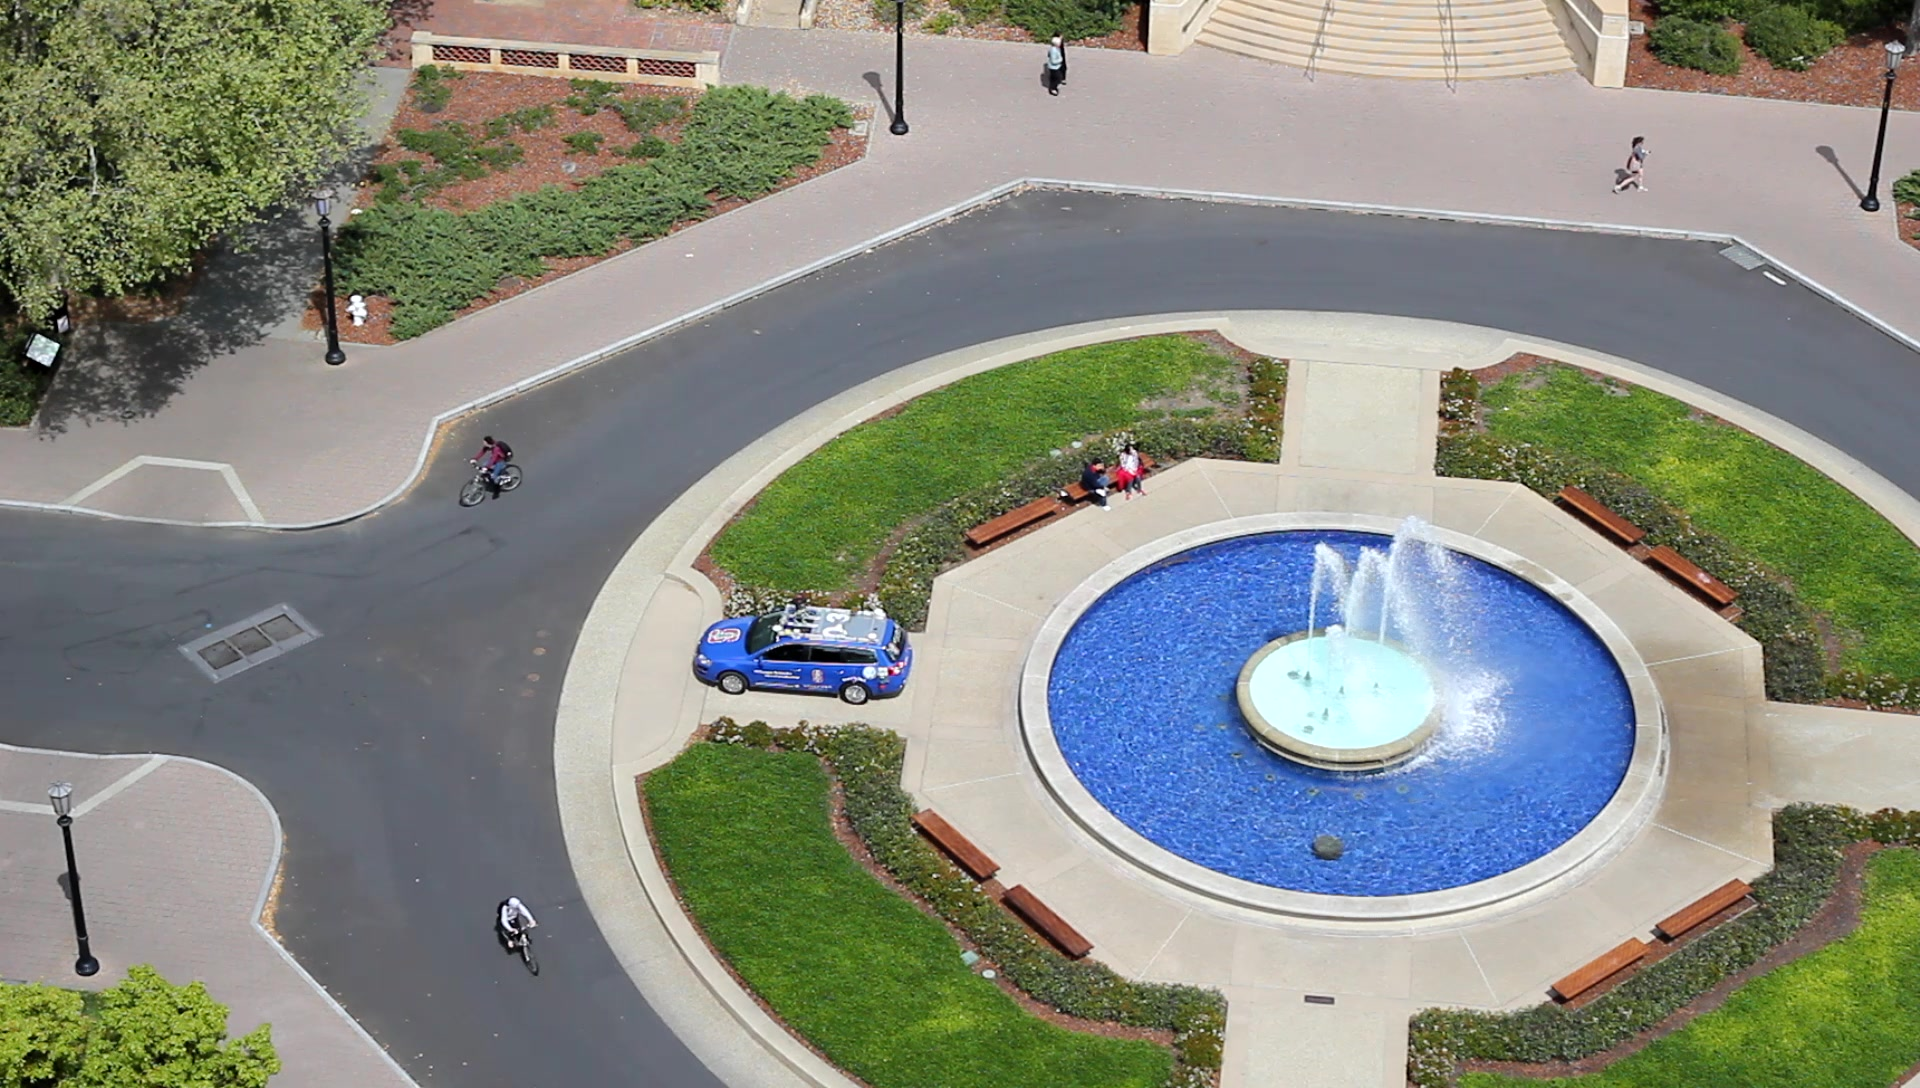
\epsfig{file=figs/campus_000042.eps, angle=0, width=1\linewidth, clip=}
%\caption{\label{fig:campus_000042} a) Input image frame.}
%\end{minipage}
%\addtocounter{figure}{-1}
%\begin{minipage}[b]{0.37\linewidth}
%\centering
%\epsfig{file=figs/RoIs_campus_000042.eps, angle=0, width=1\linewidth, clip=}
%\caption{\label{fig:campus_000042} b) Regions of Interest generated by Saliency Model.}
%\raggedright
%\epsfig{file=figs/RoIs_campus_000042.eps, angle=0, width=1\linewidth, clip=}
%\caption{\label{fig:campus_000042} c) Objects classified by HMAX Model.}
%\end{minipage}
%\end{figure*}

%Memory
Increase in computational power of most state-of-the-art systems has resulted in memory bottlenecks becoming a more and more important from the point of view of performance and energy constraints in the system.
In this section, we briefly describe the role that memory design has to play in our vision-based accelerator system.

\subsection{Motivation}
Memory is an important component of almost all computer-based systems. Given the increase in cloud-computing and server farms, the scalability in terms of power and performance of memory devices has become an important design consideration. Due to it's low-cost per bit, the dynamic random-access memory (DRAM) has become ubiquitous in most commercial applications. However as densities increase, the power wall is becoming an increasingly severe problem. Figure~\ref{fig:refreshTrends} shows the increasing power consumption across different DRAM densities. More crucially, the refresh component in the DRAM is becoming a major source of concern. 
Considerable work has gone into the area of reducing refresh power consumptions. Some have used scheduling policies~\cite{Stuecheli2010}, some have used retention profiling~\cite{Liu2012}, while others have used software techniques~\cite{Liu2012}. In~\cite{Nair2013}, the authors use a refresh pausing mechanism to exploit idle cycles in memory. In~\cite{Mukundan2013}, Fine Grained Refresh (FGR) for DDR4 DRAM systems is analyzed.  

%\begin{figure}[ht!]
%\centering
%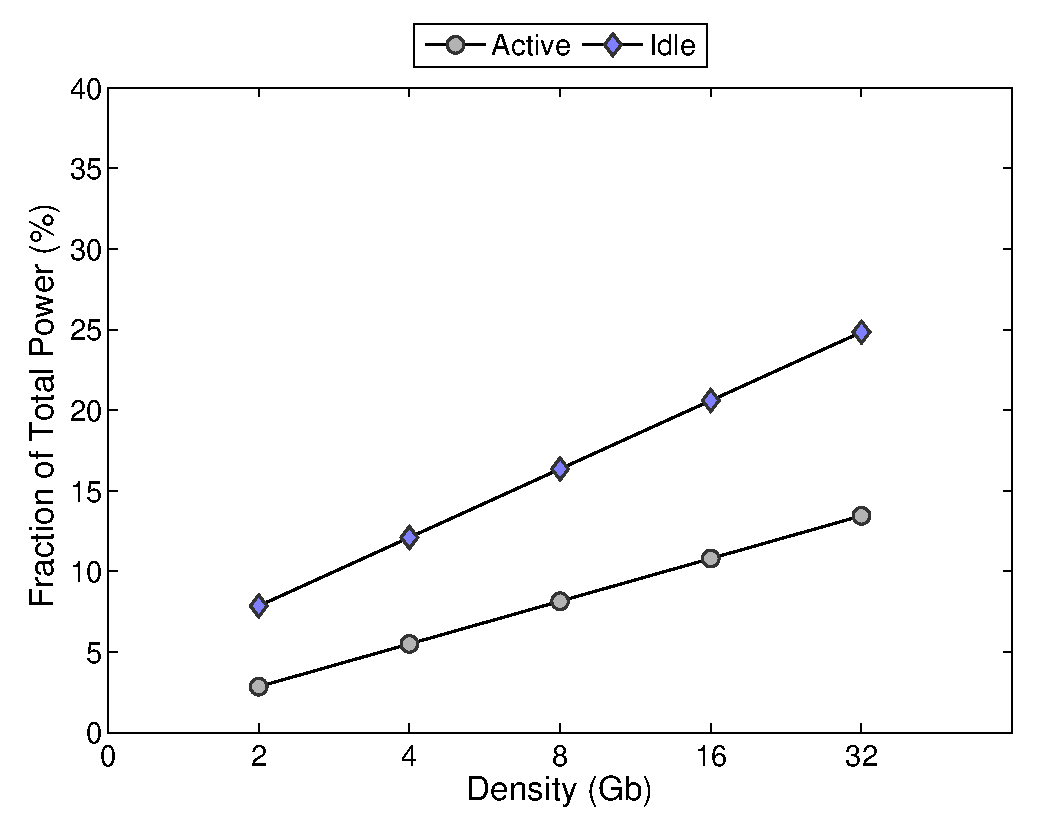
\epsfig{file=figs/RefreshTrends.eps, angle=0, width=1\linewidth, clip=}
%\caption{\label{fig:refreshTrends} Trends in the distribution of DRAM power- The refresh component increases with each generation.}
%\end{figure}

\begin{figure*}[ht!]
\begin{minipage}[b]{0.36\linewidth}
\raggedleft
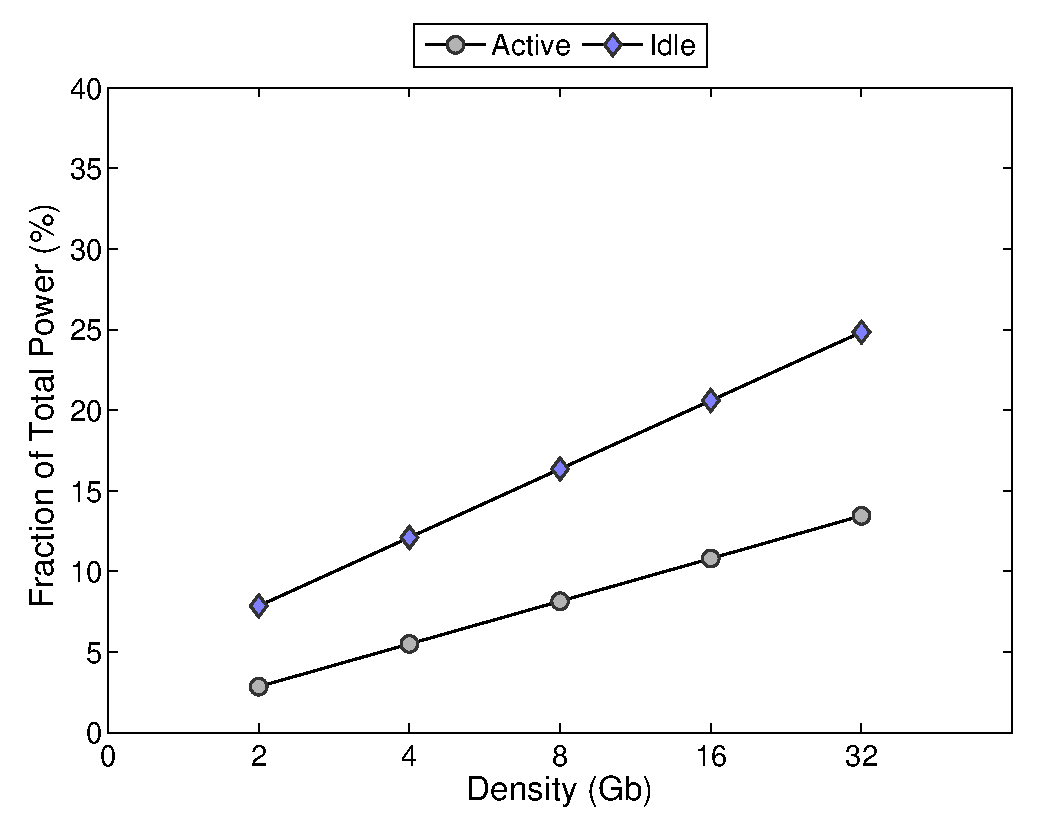
\epsfig{file=figs/RefreshTrends.eps, angle=0, width=1\linewidth, clip=}
\caption{\label{fig:refreshTrends}a) Trends in the distribution of DRAM power- The refresh component increases with each generation.}
\end{minipage}
\addtocounter{figure}{-1}
\begin{minipage}[b]{0.37\linewidth}
\centering
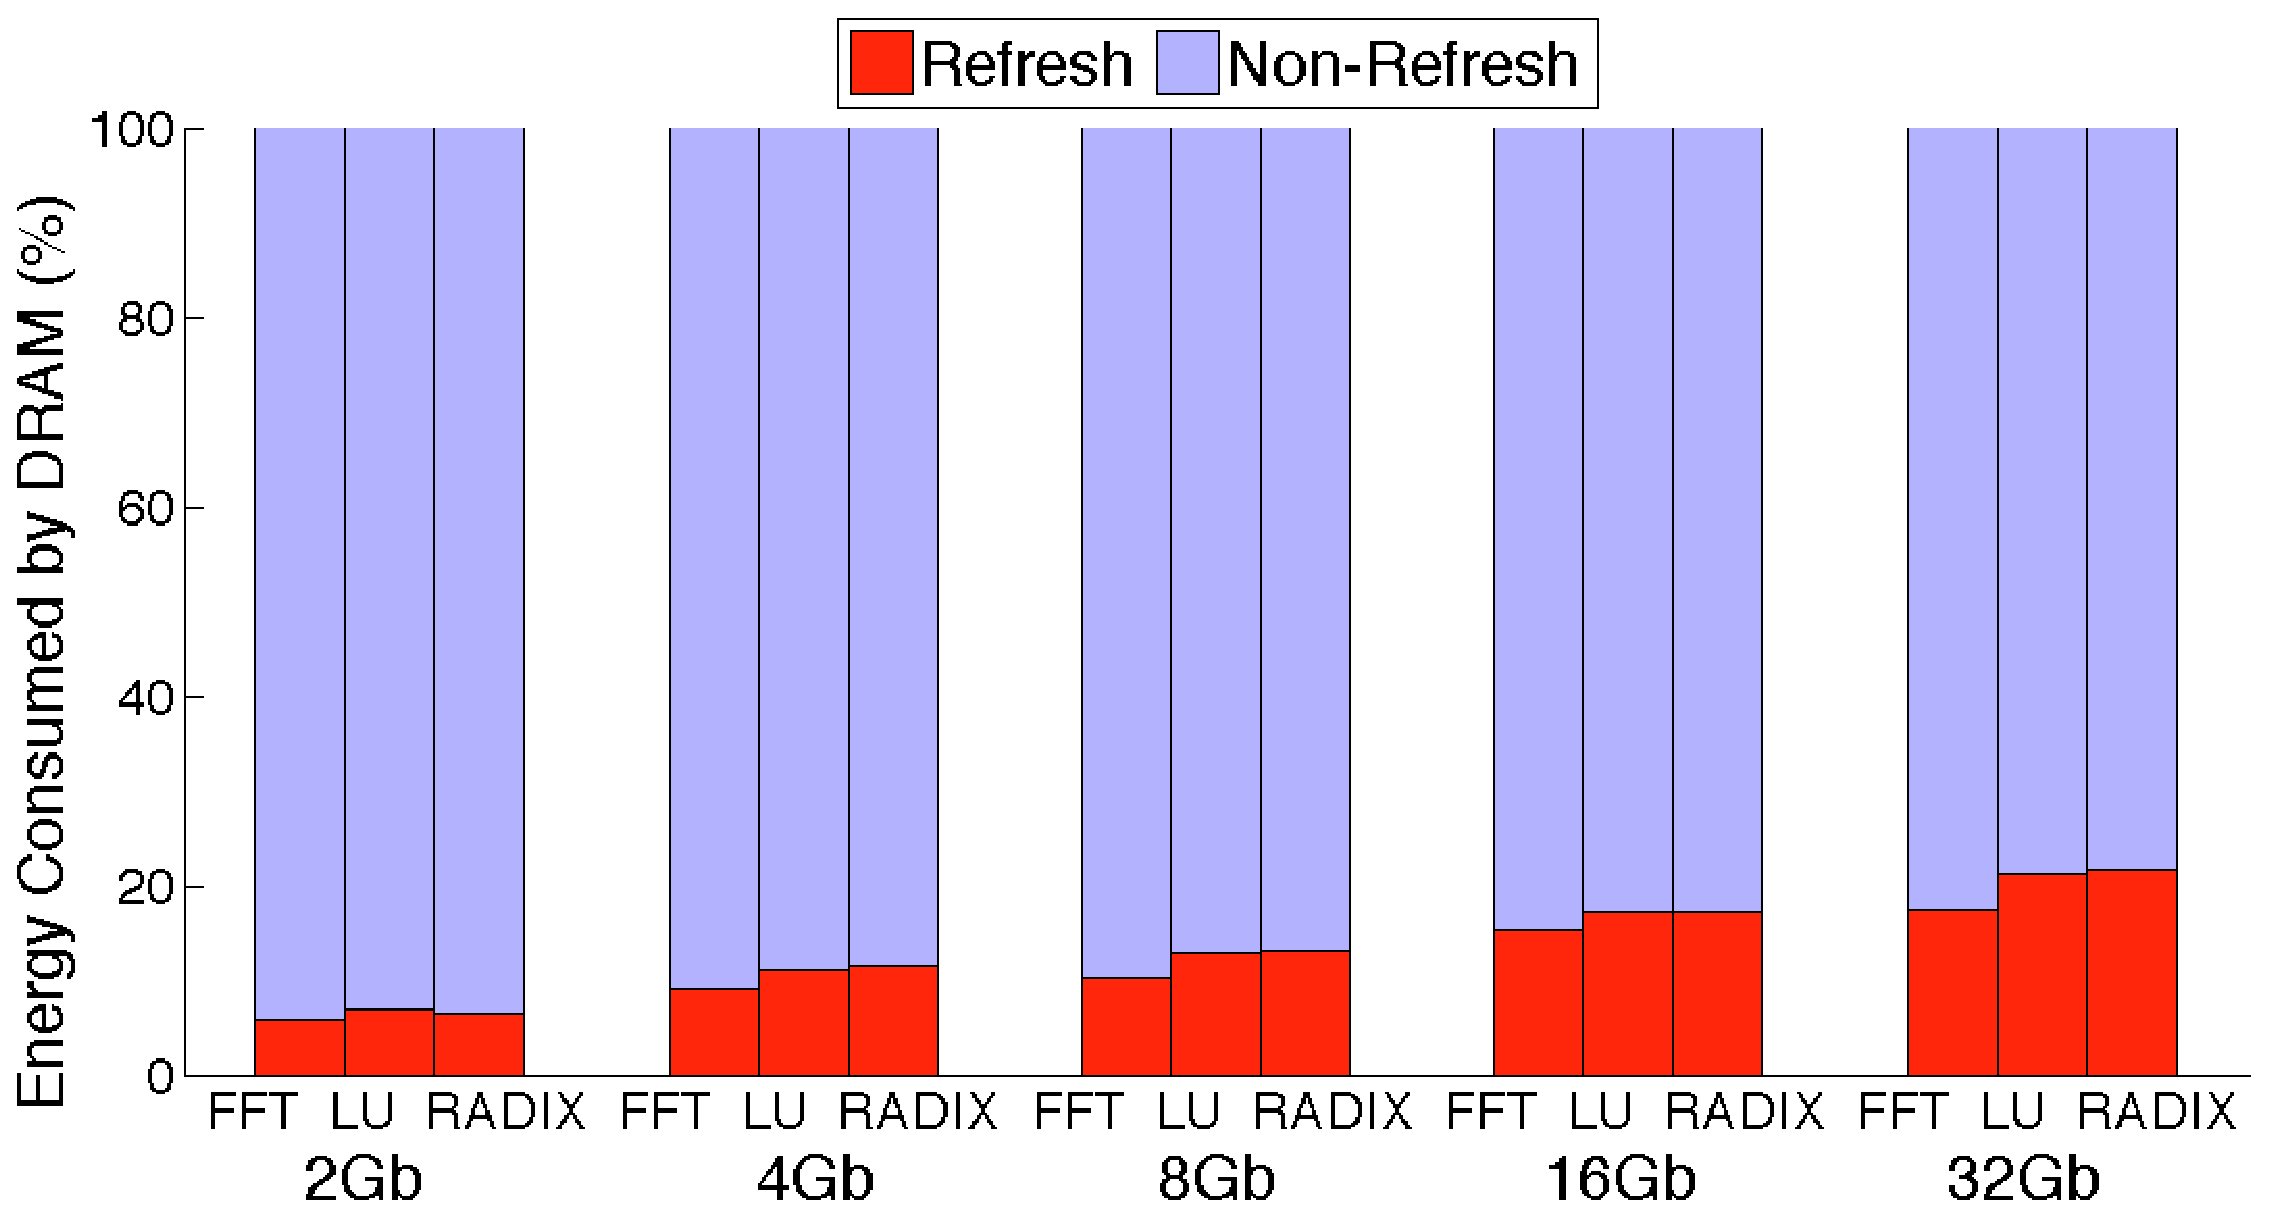
\epsfig{file=figs/DRAMEnergy_Kernels.eps, angle=0, width=1\linewidth, clip=}
\caption{\label{fig:refreshTrends}b) Refresh energy distribution in Kernel computations}
\end{minipage}
\addtocounter{figure}{-1}
%\begin{minipage}[b]{0.25\linewidth}
%\raggedright
%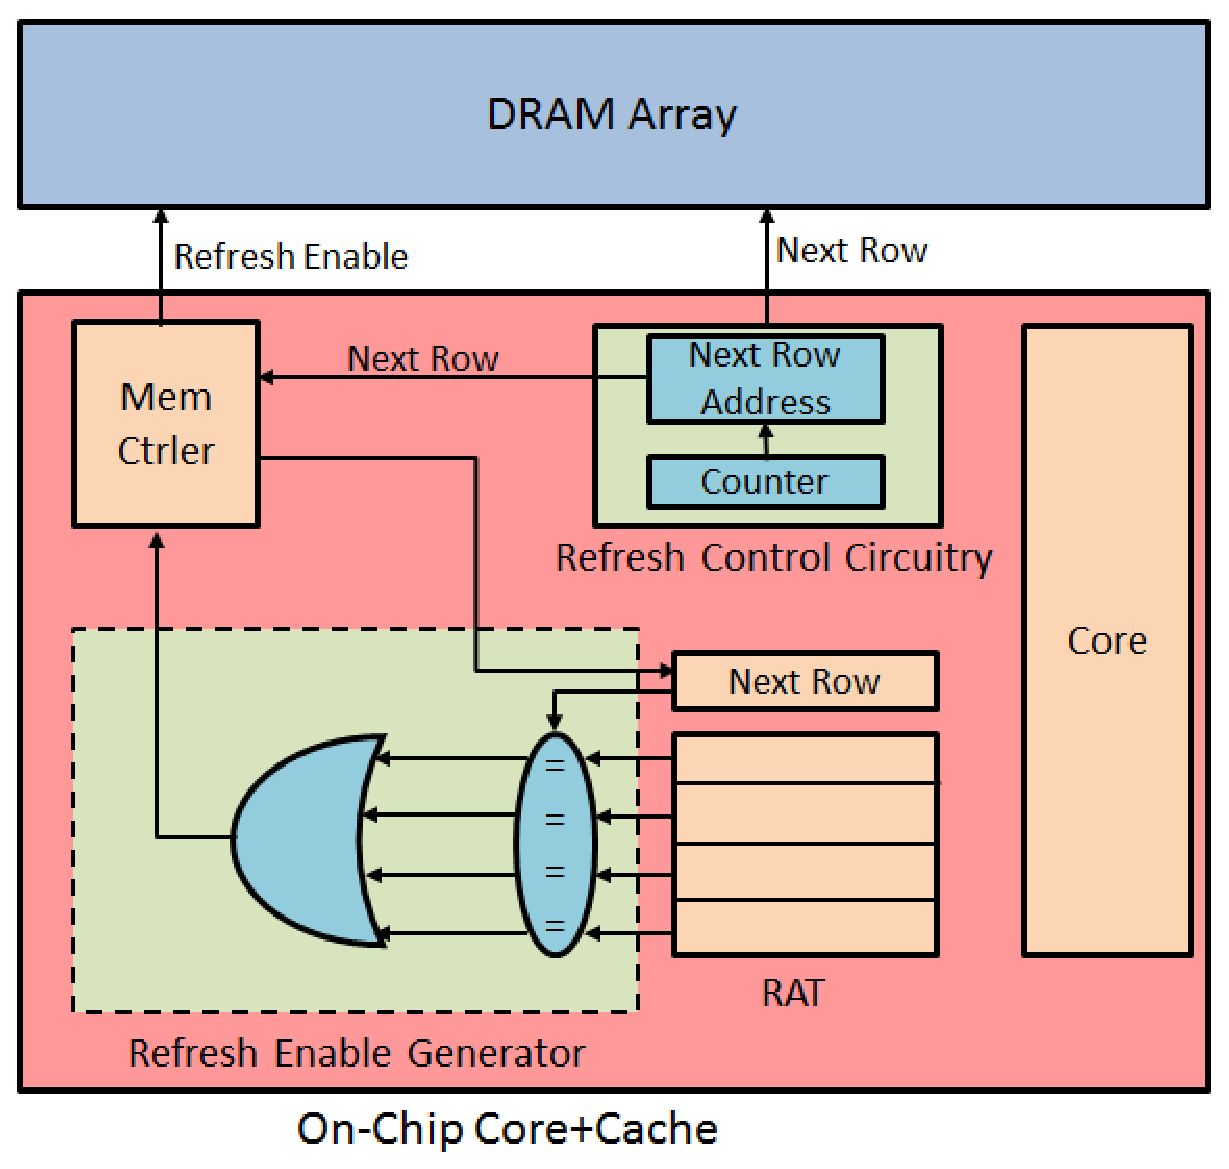
\epsfig{file=figs/refresh_circuitry.eps, angle=0, width=1\linewidth, clip=}
%\caption{\label{fig:reva}c) Design of REVA block}
%\end{minipage}
\end{figure*}

\subsection{DRAM Memory Organization}

DRAMs are organized into a series of hierarchical structures in order to exploit the potential for parallelism across accesses. The DRAM consists of one or more memory channels, each one of which has a dedicated memory controller. Each channel comprises of several ranks. Instructions can be issued to the DRAM at the rank level granularity. Each of these ranks are further subdivided into banks. A bank is a logical organization representing an independent memory array and consists of several rows. In general, each row is designed to hold a page of memory (2-4KB).

\subsection{Refresh Operation in DRAMs}
The defining attribute of DRAMs, in comparison to other memory technologies like Static RAMs and Hard Disks is the temporary nature of the data stored in it. Since a DRAM cell simply comprises of a single transistor-capacitor combination, the data is retained for only as long as the capacitor can hold the charge injected into it during a write operation. As a result it is essential to periodically refresh the data in each cell in order to maintain the integrity of the stored data. A refresh operation simply involves reading a row of data and writing it back from the sense amplifier. The write operation restores the charge in each DRAM cell capacitor to its original level. This refresh operation is handled by a built-in refresh controller. The memory controller periodically issues commands to carry out refresh to each rank.

The exact row to be refreshed and the corresponding bank are determined by the refresh controller. Most standard DRAM cells are architected with a 64~ms refresh window ($t_{REFW}$), that is each cell must be refreshed at least once every 64~ms. According to JEDEC SDRAM standards~\cite{jedec-sdram-standards}, a DRAM device can issue a maximum of 8192 refresh commands within this refresh window, leading to a refresh command being issued every 7.8$\mu$s ($t_{REFI}$). Consequently, increasing the number of rows per bank would necessitate multiple rows to be refreshed per command. The refresh controller keeps track of the address of the last row to have been refreshed so that the subsequent refresh command can enable it to issue refreshes to the next group of rows.

The major drawback of DRAM technology is the additional overhead in performance and power on account of the refresh operation. A single refresh command to a row causes the entire bank of the DRAM to stall. Hence several techniques have been incorporated into the DDR protocols to minimize overlaps between read/write and refresh commands.

Each refresh command issued by the memory controller is appended to the command queue along with other read and write commands. Depending on the read and write traffic, it is possible to delay the refresh commands so as to reduce stalls due to the refresh operation preventing the read or write from being issued to the memory. 



\section{System Architecture}
\label{sec:architecture}			%1
%Architecture
%In this section we describe in detail the system architecture, in particular the memory hierarchies along with the data mapping and refresh policies that we adopt.

\begin{figure*}[ht!]
\begin{minipage}[b]{0.36\linewidth}
\raggedleft
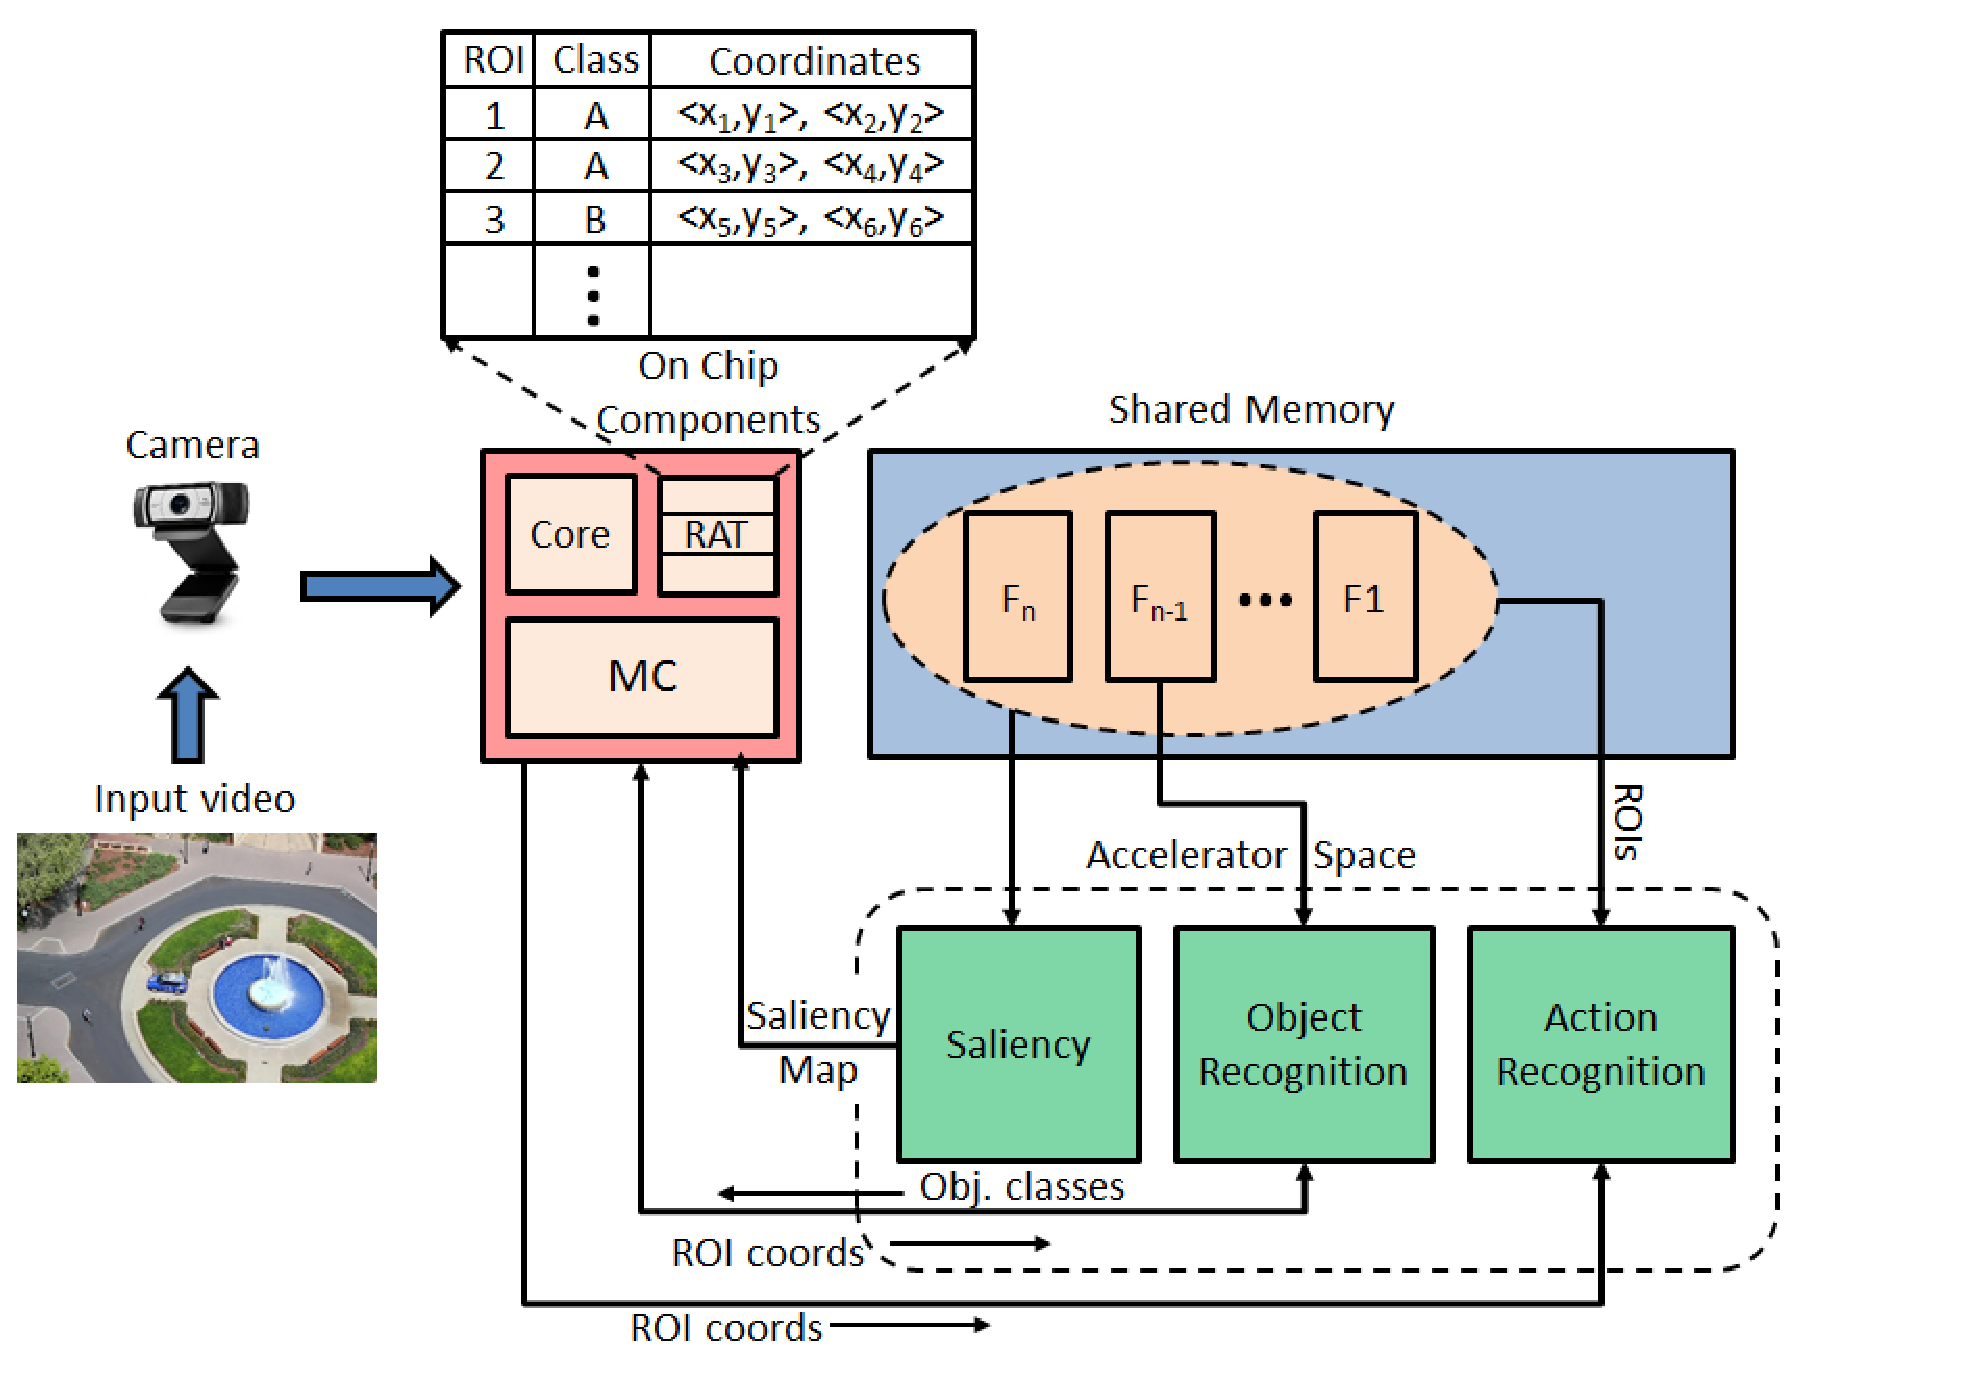
\epsfig{file=figs/baseline_arch.eps, angle=0, width=1\linewidth, clip=}
\caption{\label{fig:reva}a) Baseline architecture}
\end{minipage}
\addtocounter{figure}{-1}
\begin{minipage}[b]{0.37\linewidth}
\centering
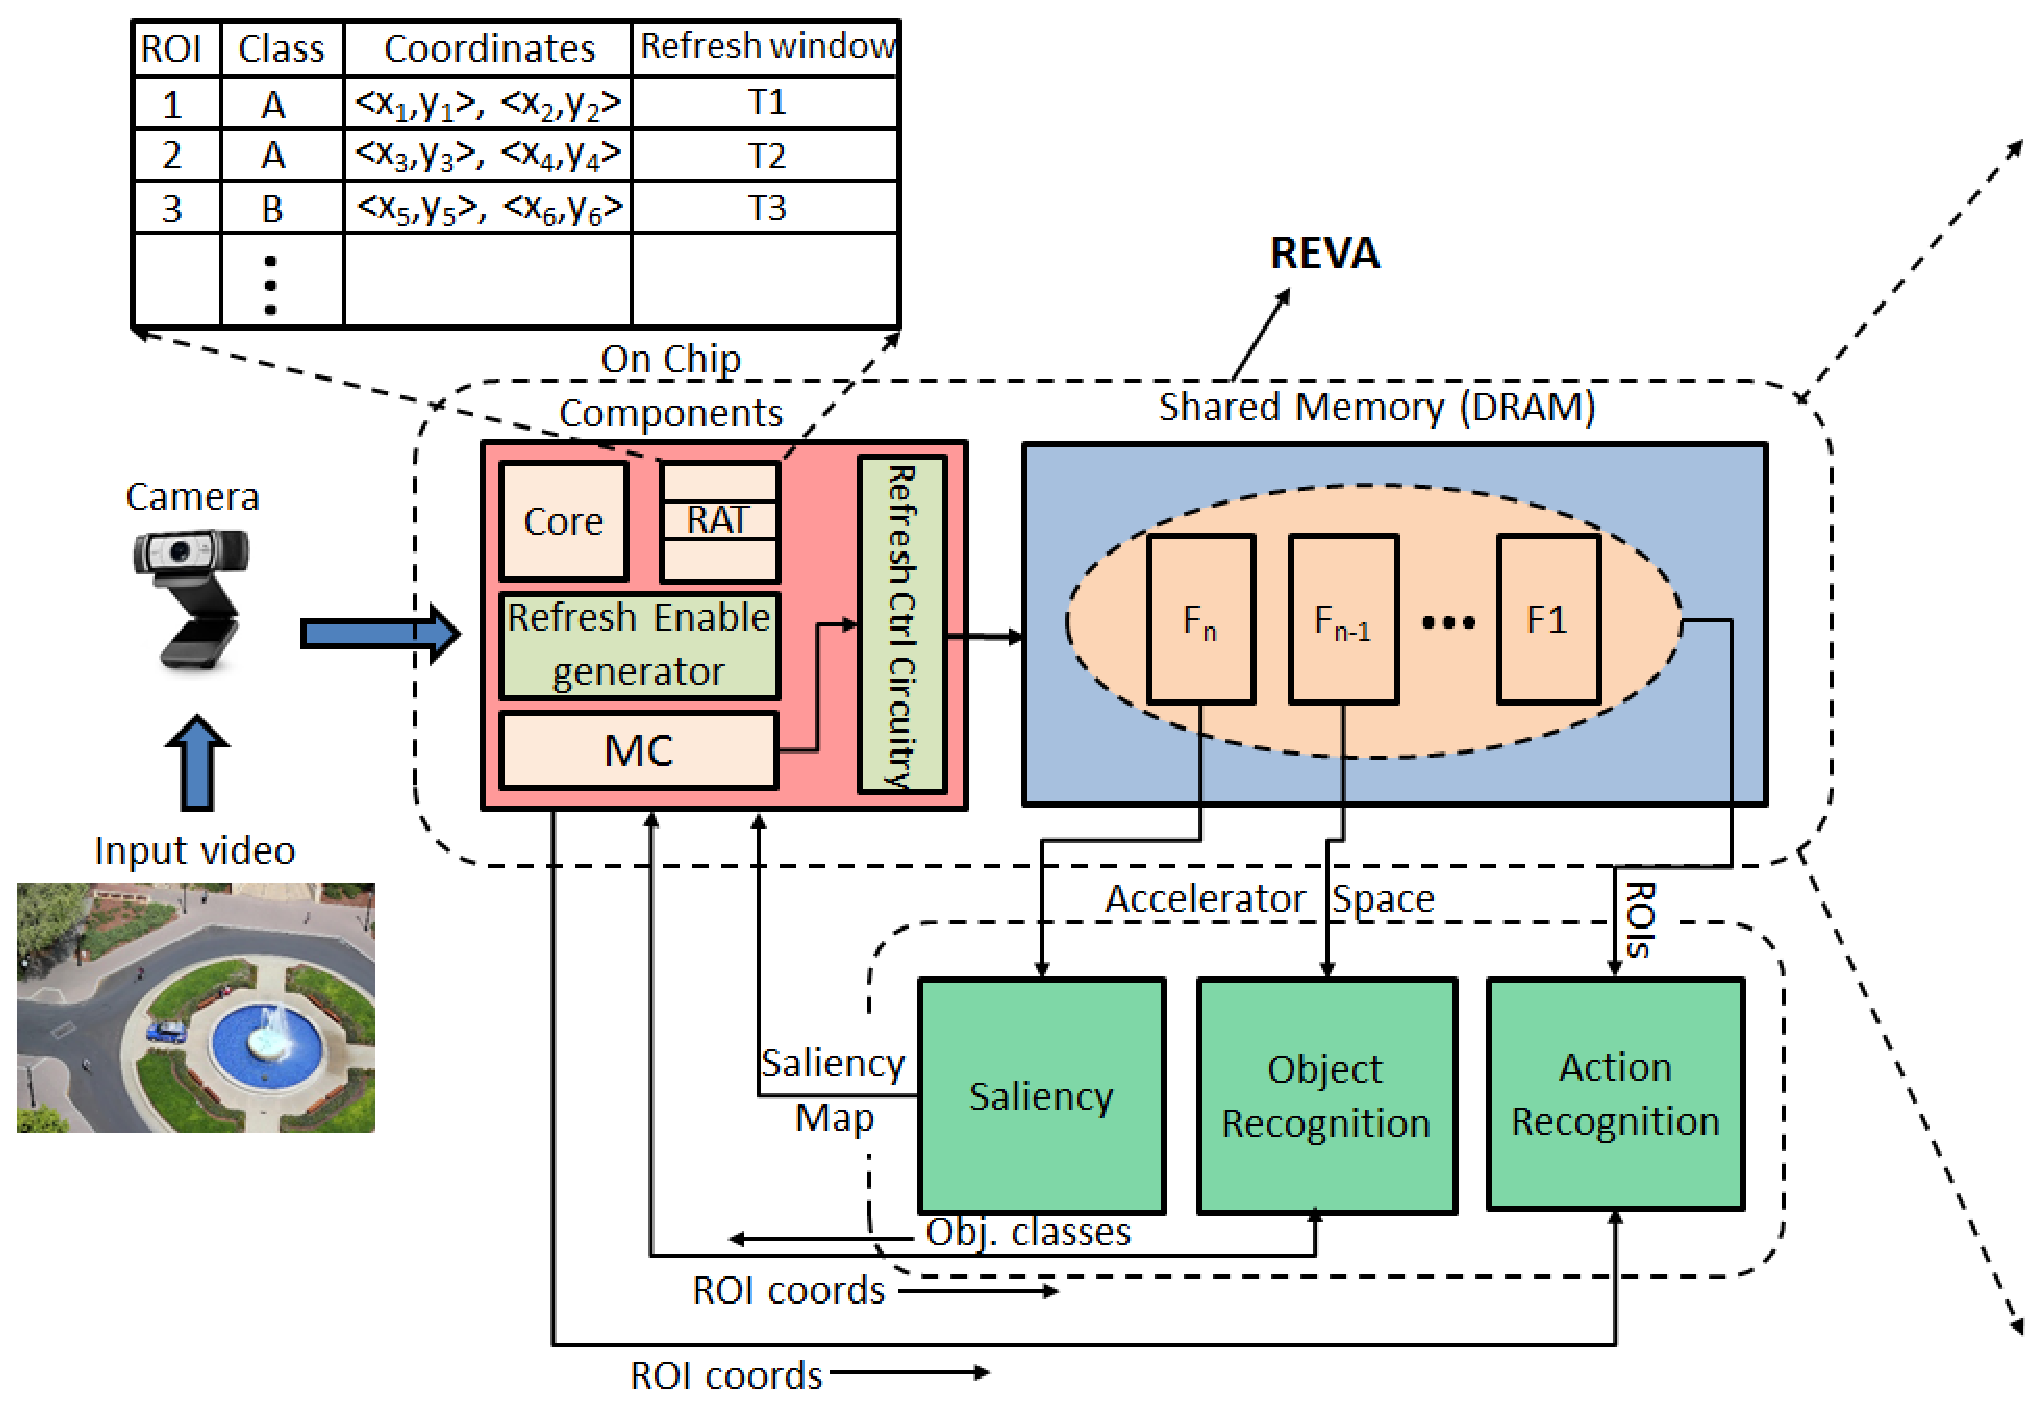
\epsfig{file=figs/reva_arch.eps, angle=0, width=1\linewidth, clip=}
\caption{\label{fig:reva}b) Architecture of Proposed System}
\end{minipage}
\addtocounter{figure}{-1}
\begin{minipage}[b]{0.25\linewidth}
\raggedright
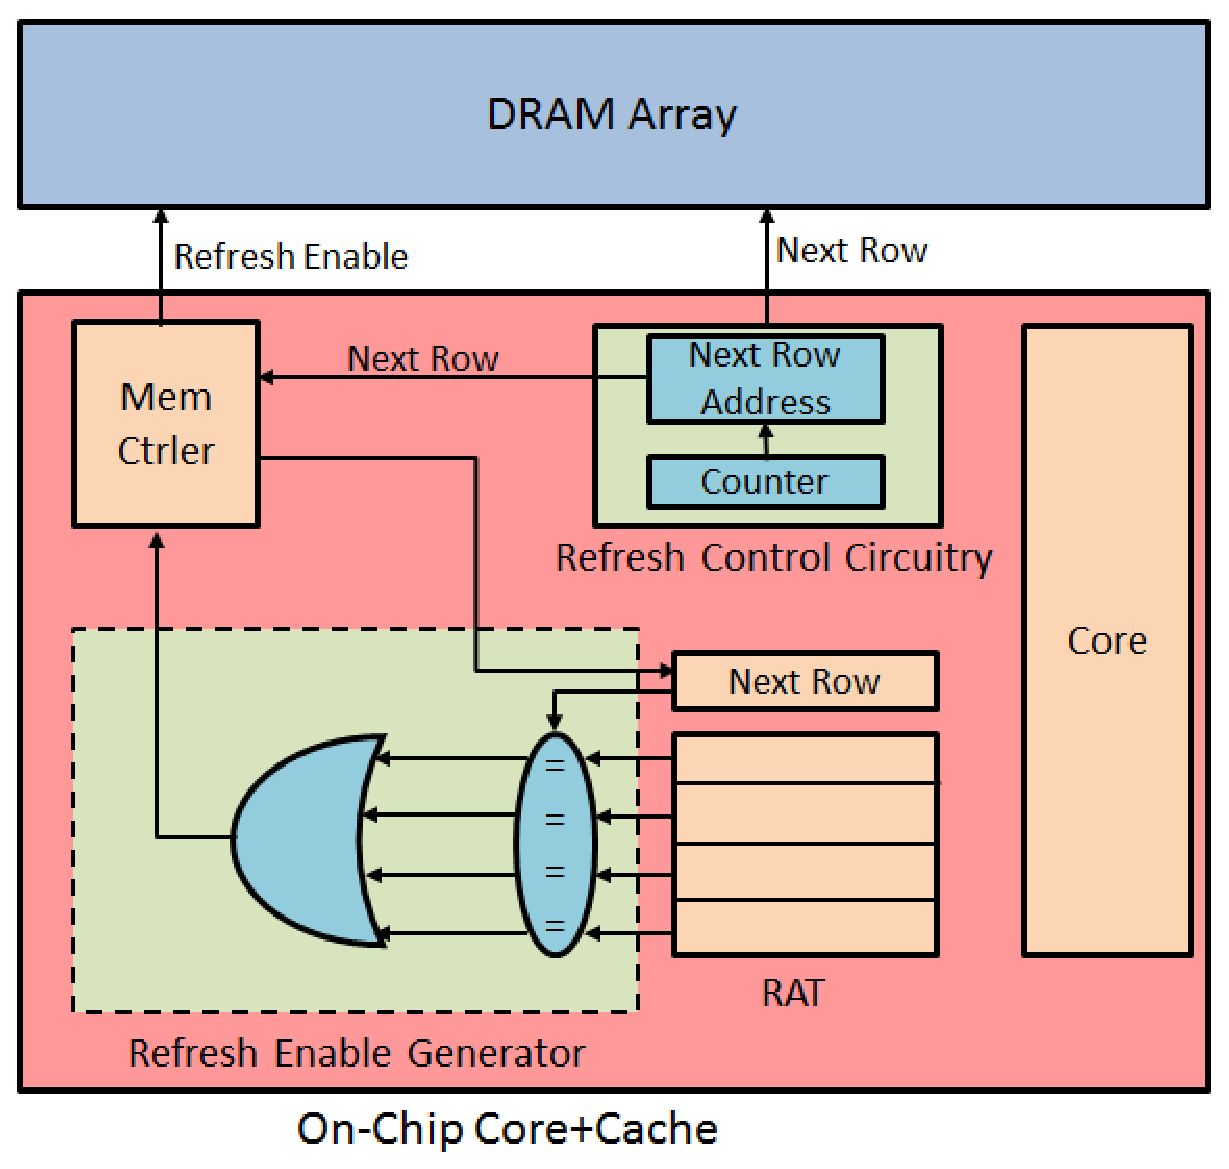
\epsfig{file=figs/refresh_circuitry.eps, angle=0, width=1\linewidth, clip=}
\caption{\label{fig:reva}c) Design of REVA block}
\end{minipage}
\end{figure*}


Figure~\ref{fig:reva}a) illustrates the baseline architecture for the vision analytics-based system. The input video is captured by the HD camera at a rate of 30 frames/s. 
These frames are stored in the off-chip DRAM, as shown in the figure. These frames are then read by the saliency accelerator and a saliency map is computed \emph{Saliency Map}. This saliency map is then used to compute the RoIs by the CPU. The Object Recognition accelerator classifies the objects in each ROI as belonging to a certain class. The Action Recognition Engine requires a series of consecutive frames to classify the exact action being carried out. Since each of these frames over the entire length of the video stored in the main memory module, there is a substantial overhead, especially in terms of refresh energy, in the baseline architecture. 

In our proposed design, shown in Figure~\ref{fig:reva}b), we recognize that the DRAM primarily serves the purpose of a stream buffer. Consequently the frames are rarely reused after processing, which may eliminate the need for refresh entirely. 
However, some accelerator operations like action recognition, require a sequence of previously stored frames to be recalled. Therefore we only need to \emph{selectively} refresh the RoIs involved in these functions. We thus propose \emph{Differential Refresh} rates based on the RoI and object class with which it has been associated by the object recognition engine.


\subsection{Differential Refresh Architecture}
As explained above, in the time duration of Refresh Cycle Time ($t_{RFC}$), a group of rows is refreshed sequentially when a refresh pulse is scheduled. A refresh pulse is sent every Refresh Interval ($t_{ref}$) time period.  When a refresh is scheduled, we keep track of the next row to be refreshed in a bank in the Next\_Row\_Address register. At the end of every refresh iteration, the content of this register is sent to the memory controller. 
We maintain an on-chip CAM structure called the \emph{RoI Address Table (RAT)} to list regions of interest (RoI) in each frame and their corresponding starting addresses and sizes. 
The RAT is analogous to the processor register file with each new RoI resulting in a new entry being written into it. Since the action recognition accelerator requires around 20 frames for a reasonable accurate classification, assuming a maximum of 4 RoIs per frame, the RAT can have a maximum of 80 entries.

When the address of the next row to be refreshed does not match an RoI address on associative search, Refresh Enable signal is set to 0. This ensures that rows of an image in a bank that do not belong to RoIs are refreshed less frequently than the rows that contain Regions of Interest. We propose two schemes to support differential Refresh rates across different sections of an image. 

Each image frame is interleaved across banks at page granularity utilizing Row Buffer Locality. The RAT is updated once the saliency accelerator computes the RoIs as shown in Figure~\ref{fig:reva}c). After a refresh iteration, when the memory controller gets the Next\_Row\_Address and a match for this is found in the RAT, a refresh pulse is sent to the command queue; otherwise Refresh Enable signal is set to low. An RoI is a 2-d rectangular tile and might correspond to different rows in different banks; the group of rows containing a portion of the RoI might also have non-RoI regions striped across multiple banks. Still, the energy overhead of refreshing non-RoI regions in rows that contain RoI is lesser than the energy overhead incurred on applying a uniform auto-refresh policy to the entire image. Since the non-RoI regions of the image are not subsequently read/written to, we allow the non-critical sections of the image to degrade with infrequent refreshes. 
On the other hand, non-image data such as code are considered to be critical and assigned a standard periodic refresh policy.
It needs to be noted that for completely stream-based processing, a no-refresh policy can be implemented allowing for corruption of the image.
%where there is a single-pass streaming access of the image, a no-refresh policy can be implemented for the entire image allowing corruption. 
This is because, a read operation inherently involves a refresh and each image row is read no more than once.
 
This scheme involves communication overhead between memory controller and the refresh controller since the address of the next row to be refreshed is sent after every refresh iteration. An alternative would be to assign fixed refresh rates for different sections of a bank. For example, the upper addresses of a bank can be configured for no refresh and the lower addresses for auto-refresh policy. However this would involve mapping the physical pages of a Region of Interest to a specific partition in the bank incurring additional OS overhead and the scheme we propose does not involve page-level mapping of Virtual Addresses of RoIs to physical pages of a partition. Also, when the saliency accelerator generates the saliency map, RoIs are not written to dedicated variable refresh frequency partitions again. Instead the saliency map computed is used to derive RoIs in input image already stored in memory and refresh frequencies are varied based on the location of RoIs. 

In order to compute the overheads due to our scheme, we use McPAT 1.0~\cite{mcpat} to estimate the power of the CAM-based RAT. Our experiments resulted in an additional power of around 2.4~mW, which is less than 1\% of the overall system power. Like the register file, the RAT is also capable of fast read and write accesses within a single clock cycle.

\subsection{Comparison with existing schemes}
Selectively refreshing the DRAM depending on data criticality has been demonstrated earlier in~\cite{Liu2011}. However, unlike their scheme which consists of a static partitioning of the memory depending on the required refresh rate, our system is capable of dynamically allocating refresh periods to stripes of rows across banks. Consequently, by interleaving data across all banks, it is possible to control the refresh rates of each individual RoI. 
This also eliminates the need for the refresh regions to be re-written into a separate section of pre-allocated memory, as in the case of~\cite{Liu2011}.

Figure~\ref{fig:reva-refresh} contrasts the two schemes described above. It can be observed that our scheme makes dynamic refresh allocation, which lends more flexibility and also reduces the need for redundant writes of the RoI.

\begin{figure}[ht!]
\centering
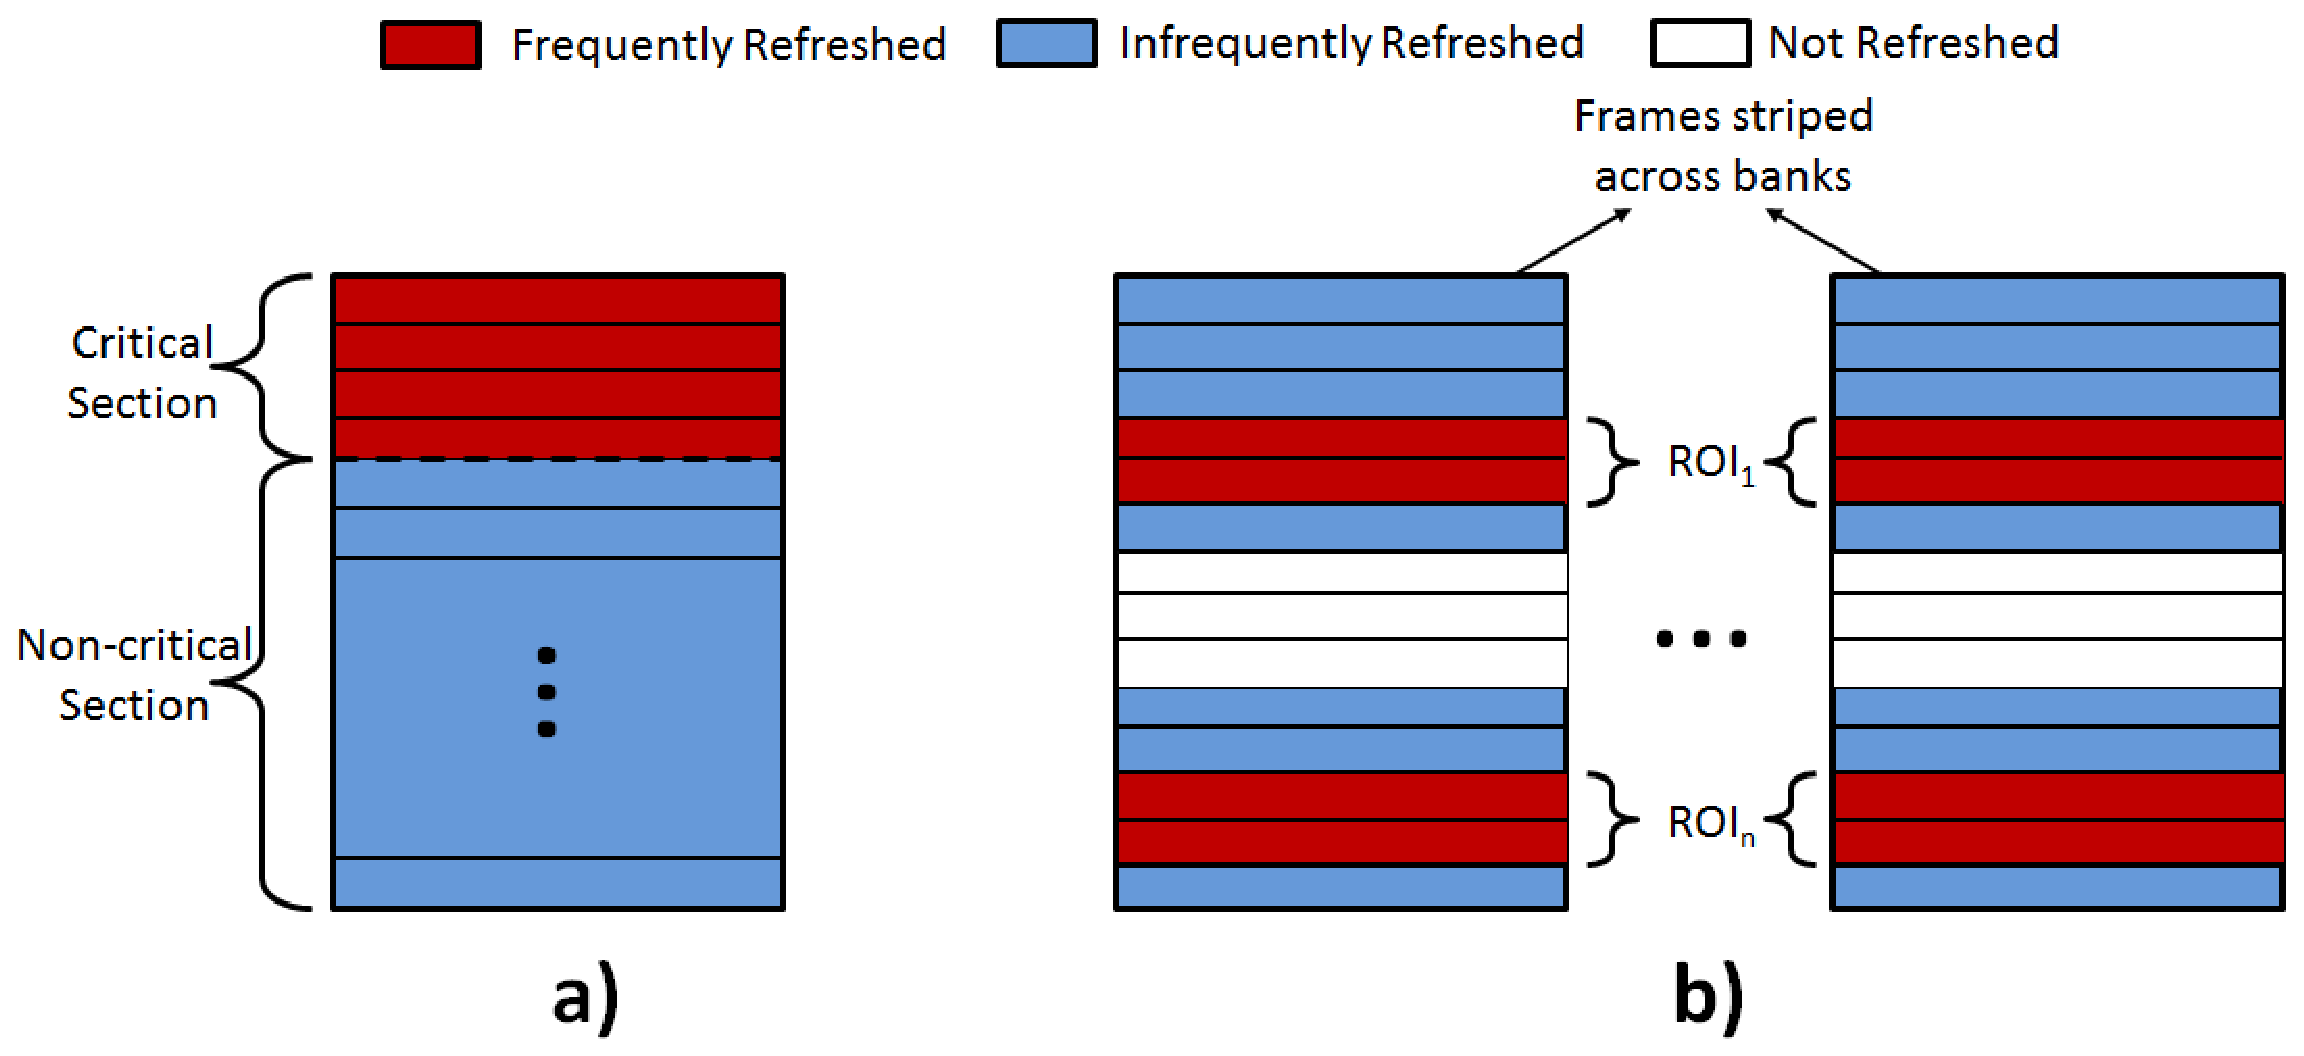
\epsfig{file=figs/reva_refresh.eps, angle=0, width=0.9\linewidth, clip=}
\caption{\label{fig:reva-refresh} Refresh mechanisms in a) Flikker  b) REVA}
\vspace{-0.2in}
\end{figure}



\section{Experimental Setup and Results}
\label{sec:results}			%1
%Results
\subsection{Experimental Infrastructure}
Figure~\ref{fig:experimental-setup} shows the infrastructure setup we used to carry out our evaluations.
We used DRAMSim2~\cite{DRAMsim2}, a cycle accurate memory simulation tool, which we customized to incorporate our refresh mechanisms. 
The input traces to DRAMSim2 were generated using the Xilinx Vivado~\cite{vivado} environment in the following manner.
The different accelerators, namely saliency, object recognitoin and action recognition, were implemented in Verilog and their output was used to generate parameters which was fed to a traffic generator.
This traffic generator outputted the memory trace comprising of read and write memory accesses.

\begin{figure}[ht!]
\centering
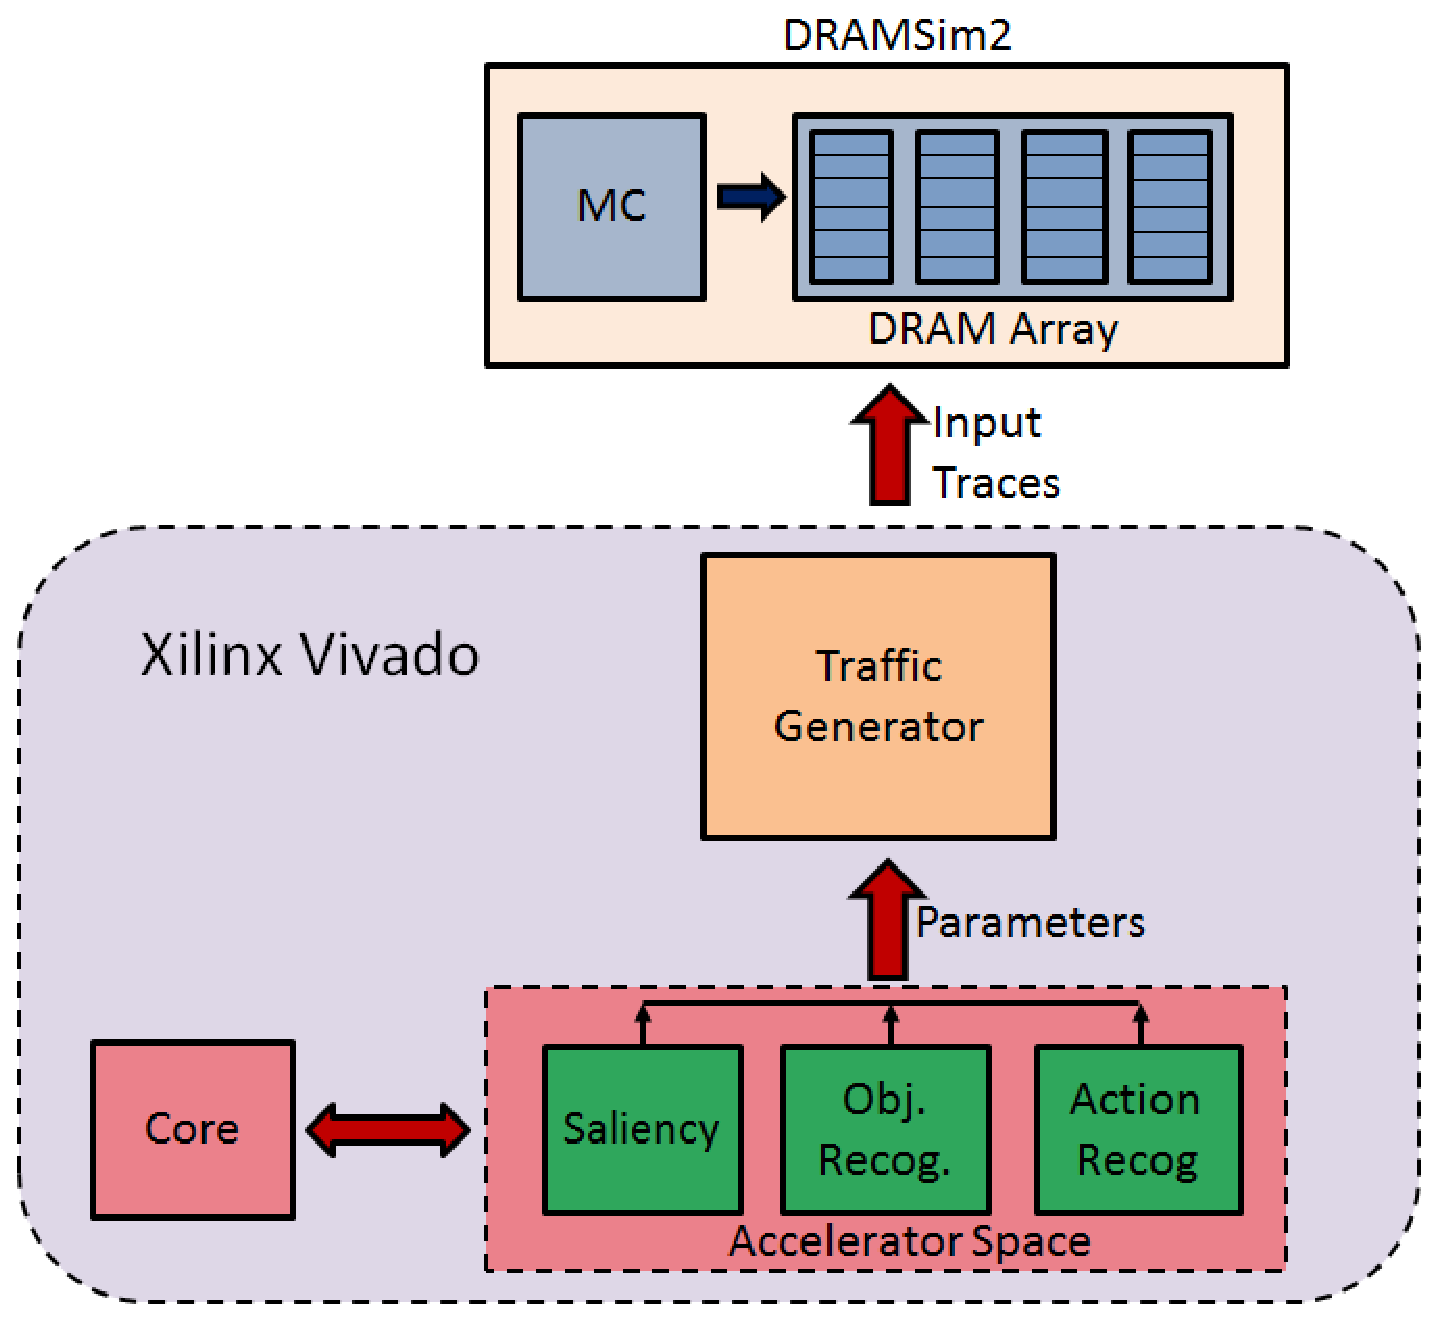
\epsfig{file=figs/experimental_setup.eps, angle=0, width=0.8\linewidth, clip=}
\caption{\label{fig:experimental-setup} Infrastructure setup}
\end{figure}

Table~\ref{tab:dram-parameters} shows the parameters used in our DRAM model, which we configured for simulation using DRAMSim2.


\begin{table}[ht!]
\footnotesize
\centering
%\vspace{-0.2cm}
\begin{tabular}{|c|c|} \hline
DRAM row & Open page\\
buffer policy & Closed after 4 accesses\\\hline
DRAM & DDR3-1600, 8 Gb, 1 channel,\\
configuration &  1 rank, 8 banks/rank \\\hline
Timing & $t_{RP}=11$, $t_{RCD}=11$\\
parameters (ns) & $t_{RFC}=350$, $t_{REFI}=7800$ \\\hline
Current & $I_{DD0}=110$, $I_{DD1}=135$, $I_{DD2P}=40=I_{DD2Q}$ \\ 
parameters (mA) & $I_{DD2N}=42$, $I_{DD3N}=45$, $I_{DD4W}=280$ \\ 
&$I_{DD4N}=270$, $I_{DD5}=215$, $I_{DD6}=12$ \\\hline
\end{tabular}
\vspace{0.1in}
\caption {DRAM parameters}
\label{tab:dram-parameters}
\end{table}

\subsection{Results}
Figure~\ref{fig:PowerResults} illustrates the total power consumption evaluated by feeding the traces generated from Vivado into DRAMSim2 for a 8 Gb based DRAM. We evaluate our scheme versus our best attempt at modeling Flikker in the given simulator. It should be noted here that when an action recognition task is triggered, a Flikker mechanism would require additional writes to move the RoIs from Non-Critical to Critical section since the action recognition would entail a 2 second video segment computation. REVA on the other hand would be dynamically capable of changing the refresh value in the RAT, thus avoiding additional writes. We also show results when we turn refresh completely off. 

\begin{figure}[ht!]
\centering
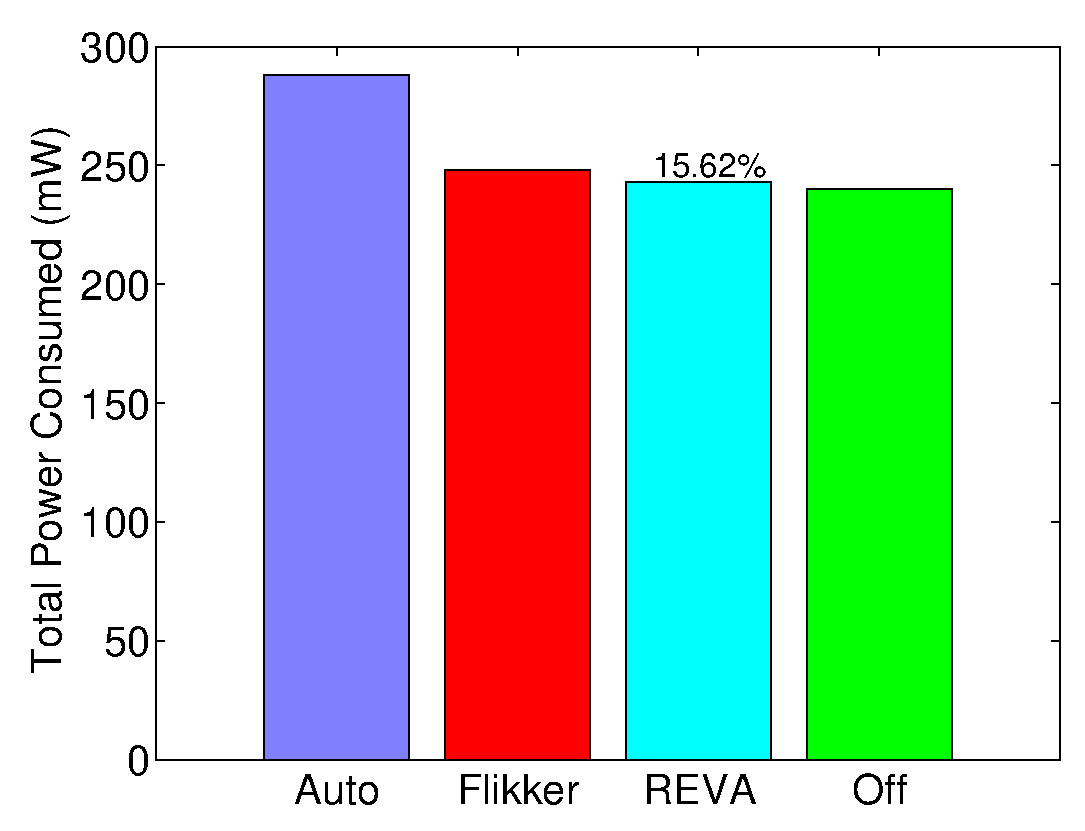
\epsfig{file=figs/DRAMPower_Improvement_8GB.eps, angle=0, width=0.9\linewidth, clip=}
\caption{\label{fig:PowerResults} Power comparisons for different schemes.}
\end{figure}

\subsection{Sensitivity Analysis}
While it can be argued that in a purely streaming embedded system, one can completely turn off refresh, we provide a compelling reason to have a variable dynamic refresh mechanism in place. There can be instances when a burst of RoIs are generated and the object recognition accelerator cannot sustain a high throughput of generating class labels. RoIs need to be buffered in the DRAM for processing at a later stage. Similarly, an object classified by HMAX may need to be evaluated further by SIFT for object matching or sub-class recognition. Then too the object needs to be stored for a period longer than the regular DRAM refresh interval. Lastly in a multi-object scenario, if a person's action is being recognized, another classified person's actions need to be buffered so as to process at a later stage. As shown in Figure~\ref{fig:ActionRecognition}, we evaluated different configurations of action recognition on the Weizmann dataset~\cite{Weizmann}. The results indicate that a purely streaming (no overlap of video segments) configuration affects accuracy considerably (by approximately 10 \%).  

\begin{figure}[ht!]
\centering
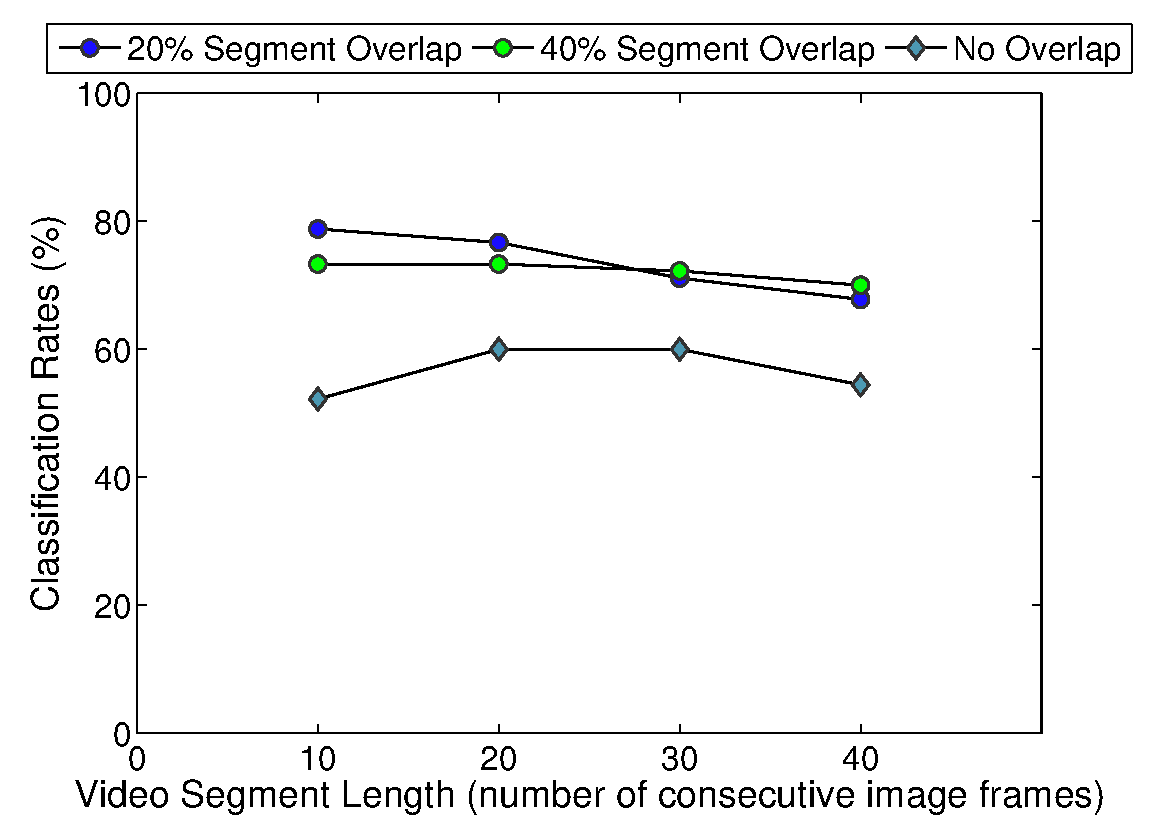
\epsfig{file=figs/ActionRecognitionAnalysis.eps, angle=0, width=0.9\linewidth, clip=}
\caption{\label{fig:ActionRecognition} Accuracy results for different configurations of video segment length and fraction of overlap between segments.}
\end{figure}




\section{Conclusion}
\label{sec:conclusion}			%1
%Conclusion



\section*{Acknowledgments}
\label{sec:acknowledgments}			%1
%Acknowledgments
This work was supported in part  by NSF Expeditions in Computing Award 1317560, and NSF award 1213052. The work was also supported by infrastructure provided by NSF Award 1205618.


%\bstctlcite{bstctl:etal, bstctl:nodash, bstctl:simpurl}
\bibliographystyle{IEEEtran}
\bibliography{IEEEabrv,library}

\end{document}

